\section{Evaluation}
\label{sec:exper}


In this section, we present some experimental results
from the proposed framework.

\subsection{The Experimental Setup}
We implement and test the performance of the algorithms 
under different potential attacks.
All algorithms are implemented with C and all
experiments are conducted on Core PC with 2.0 GHz
CPU and 2 GBytes of memory running the Ubuntu 12.04 operating system.
%All editing operations on the digital road maps in Shapefile are
%accomplished by SAGA software \cite{sagaurl}. 

\begin{figure}[ht]
\centering
\epsfig{file=images/region.eps,width=0.5\columnwidth}
\caption{Twin-Cities Seven-County Road Map}
\label{fig:region}
\end{figure}

%\subsubsection{GIS Spatial Data Set}

%We use the Minnesota (MN) state base map of the Minneapolis-St. Paul 
%Metropolitan area as our GIS spatial data set to analyse the performance 
%of our proposed watermark algorithm. 
We use MN state base 
map of seven counties, namely, Anoka, Carver, Dakota, Hennepin, Ramsey, Scott, 
Washington, as our real data set for this experiment. 
%This base map we select is in ShapeFile format\cite{shapefileurl}, 
%specifically in the Measured Polyline type. 
In this data-set, there are in total 415,651 line segments
and 372,466 different points. Figure \ref{fig:region} shows the visual map
of digital data for these seven counties. This data set can
be downloaded from the MN/DOT web site\cite{mndoturl}. 
%Since the data
%set is in the ShapeFile format originally, we need first to
%transform it into text format and manipulate this text file in our algorithm.

%\subsubsection{Experiment Design}

%The purpose of this experiment is to analyse the performance of our proposed 
%watermark approach under different attack scenarios. 
%An original GIS spatial 
%data set, watermarks, and secret keys are fed into the watermark insertion 
%module and watermarked GIS spatial data is output. Then this watermarked data 
%set is attacked by different possible attacks that are differentiated by 
%different attack parameters. Finally, the attacked watermarked data and the 
%secret keys used in the watermark insertion module are input into the watermark 
%detection module to extract the inserted watermarks that will be used to check 
%whether the GIS spatial data set has been used illegally.
%

%\KZ{%Say clearly how you obtain the cropped and merged and noise test data set.
%Show some example snapshot if possible.\\
%For each original map, one watermarking scheme and one attack method,
%there are basically three things we need to measure:\\
%1) amount of distortion added by the watermarking;\\
%2) detection accuracy;\\
%3) execution time for insertion and for detection\\
%With the about result data, we can probably design various ways to showcase it, e.g.,
%average over different maps, or a scatter plot of times, or correlation plot between
%distortion and accuracy, etc.
%}

In order to evaluate the robustness of our watermarking algorithms (which is called
Jiang in the rest of this section), we illustrate 
the performance of our proposed watermark approach under different attacks with 
different settings. In this part, we compare the proposed approach with two other 
watermarking algorithms proposed by Pu\cite{PuDJ06} and 
Voigt\cite{Voigt:2003}. Both methods are blind watermarking algorithms and provide 
some resistance to crop attack. We control the accuracy lost of the experiment data 
caused by different methods and compare the performance of them under noise attack, 
crop attack and merge attack. In this section, ``crop ratio'' and ``merge ratio'' 
mean the area ratio we crop from the total watermarked map. We set $\xi$ as 0.95.

\subsection{Performance under Noise Attack}
Noises are added to randomly selected subsets of watermarked maps. Meanwhile, to 
keep the usability of a map, those subsets could not take too much proportion of the total 
map. In this experiment, we watermark the map of St. Paul area and attack the watermarked 
map with some random Gaussian noise, perturbing the map with different accuracy lost. 

In this noise attack experiment, we watermark the map with algorithms of Pu\cite{PuDJ06}, 
Voigt\cite{Voigt:2003} and Jiang in certain 
distortion. After that we attack the watermarked maps with different noise distortion. 
For each noise distortion, the noise will be added in different methods for 20 times. 
For all three methods, the noise added is ``exactly'' the same each time.
At last, we detect the watermark and calculate detection accuracy for three algorithms. 
We set distortion $\delta_w$ added by the watermarking as $10.5\times 10^{ -6 }$ (Jiang), 
$10.8\times 10^{-6}$ (Voigt) and $9.8\times 10^{-6}$ (Pu). Take the size of map into consideration,
these distortion can be deemed at the same level. On the other hand, the noise distortion 
$\delta_n$ is changed from $5.12 \times 10^{-3}$ to 
$2.56 \times 10^{-2}$. Actually, $\delta_n$ here is large enough that almost changes all 
vertexes of the map. Figure \ref{fig:noise} shows the results.
%\KZ{%Does it make sense to have different distortion levels for three
%experiments? 
%I think we want to compare the trend against $\delta$ for
%these three experiment to show that our method is less sensitive to distortions.
%Also I think we want graphs/tables that show how performance varies with
%different $\delta$ (noise) and different $\delta$ (watermarks). These two
%$\delta$'s are different but it will be good if we can show both in one graph.}
%\KZ{It's called ``distortion'', not ``distortion distance'', because 
%it's measured globally for the whole map and not for each individual points.
%Are you going to apply the noise to only subset of the points or 
%all the points?
%In any case, you need to make sure you apply the *exactly* the same distortion
%(i.e., same distortion at the same point) to the map for each of the 3 methods, though 
%the watermarks for these 3 methods maybe different.}
 


\begin{figure}[th]
\centering
\epsfig{file=images/noiseattack.eps,width=0.6\columnwidth}
\caption{Performance under Noise Attack %\KZ{Why is Voigt almost the same
%as us? Why is Yu-Chi so bad? Btw, it should be Yu-Chi, not Yuchi in all
%the graphs.}
}
\label{fig:noise}
\end{figure}

In this experiment, we set the standard of positive detection as correctly
decide the whole map is watermarked. However, in fact, according to the 
detection method of our algorithm, some more assistance can be obtained.
Even the whole map is failed to be detected, the result could be a series
of sub-regions that is suspicious. 
The results show that our algorithm successfully survived noise 
attack. On one hand, we watermark certain bits which will not be directly affected by 
the noise if perturbing for individual vertex is under certain strength. 
Meanwhile, even the perturbing for individual vertex is powerful enough, 
$\theta $ and the hash function of $sl$ in in partition and insertion 
algorithms provide a good tolerance for it. 
   
\subsection{Performance under Crop Attack}
%\JK{For crop attack, I plan to implement three experiments.\\ 
%1). Watermark a map in certain strength and crop it into seven county 
%maps. Then I will give a table of detection confidence of each cropped 
%map. \\ 
%2). I will watermark the map with different distortion distance, and then 
%crop them to a certain ratio, e.g. 1/2, for 20 times. Then the result 
%will be a ``detection accuracy-distortion'' figure. In this experiment,
%a ``time-distortion'' figure can also be obtained.\\
%3). From the 2) experiment, we select the minimum ``distance'' to watermark
%a map, then crop it in different ratio. For each ratio, 20 different cropped
%maps will be detected. The result will be a ``Detection accuracy-crop ratio'' 
%figure for all three algorithms. }
%\KZ{%How do you crop into 7 maps, one for each county? I thought you use
%an automatic way of cropping now which means you can only crop out rectangular
%maps? 

%For (2) it can be a scatter plot, x-axis been distortion, y-axis being
%detection accuracy. The time-distortion can also be scatter plot (see Zhixian's
%paper for an example) Also for (2) you can have one plot for each algo, or
%plot all three together together on one plot but using different color or 
%different point styles. For (3) I don't understand what you mean by
%minimum ``distance''. But I sort of see the meaning of detection accuracy
%vs. crop ratio. This experiment shows how strong we are in ``massive crop''
%attacks, right? I think all 3 experiments are good!}

In our experiment, on one hand, each county out of seven is selected to be 
detected. On the other hand, some certain proportion of the map is selected 
to evaluate the performance of our algorithm. 

In this experiment, the parameter $\theta $ is set as 30,000.0 
($\delta_w=10.5\times 10^{ -6 }$) and the square side 
length is 100.0 for both insertion and detection. We partition the whole map 
of Minneapolis-St. Paul Metropolitan area. Then the watermarked map is split 
according to the boundary of different counties. After that, we impose our 
watermarking algorithm on these ``partial'' maps, trying to decide whether the 
maps are parts of our original map. Table \ref{tab:crop} shows the results of 
this experiment. 

\begin{table}[ht]
\centering
\caption{Crop Attack Detection}
\label{tab:crop}
\begin{tabular}{|c||c|c|c|c|} 
\hline
County & Total & Match & Confidence & Result \\\hline \hline
Anoka & 55 & 51 & 1.000 & positive\\\hline
Carver & 28 & 23 & 0.999 & positive\\\hline
Dakota & 68 & 61 & 1.000 & positive\\\hline
Hennipin & 141 & 137 & 1.000 & positive\\\hline
Ramsey & 58 & 56 & 1.000 & positive\\\hline
Scott & 29 & 25 & 0.999 & positive\\\hline
Washington & 46 & 43 & 1.000 & positive\\\hline
\end{tabular}
\end{table}

By analyzing the insertion algorithm, we can easily get the notion that the 
partition criterion $\theta $ has a large influence on the result of our watermark 
algorithm. We also design a series of experiments to figure out the influence 
of the $\theta $. In this experiment, we watermark the map with different distortion 
(\ref{equ:distort}) by adjusting $\theta $ (see Figure \ref{fig:dis}) and then select 
the crop ratio of $1/2$, $1/4$ and $1/8$ of the map to detect. Each ratio is detected 
for 20 times.  Figure \ref{fig:m} show the result of experiments. 
Insertion (Figure \ref{fig:ti}) and detection (Figure \ref{fig:td}) time 
for different distortion is also measured.

\begin{figure}[th]
\centering
\epsfig{file=images/cropmethod.eps,width=\columnwidth}
\caption{A Showcase of Crop Ratio 1/4}
\label{fig:cropmethod}
\end{figure}

%\begin{figure}[th]
%\centering
%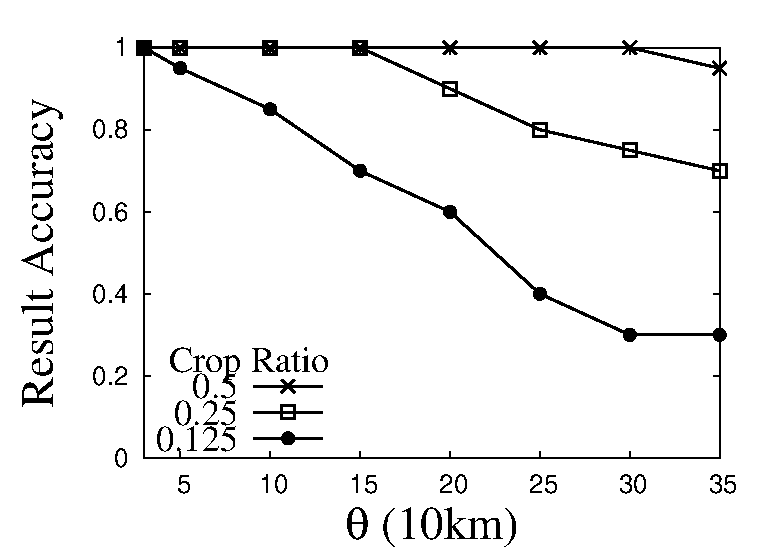
\epsfig{file=mparameter.eps,width=0.8\columnwidth}
%\caption{Performance Under Different Distortion}
%\label{fig:m}
%\end{figure}

%\begin{figure}[h]
%\centering
%\epsfig{file=mdelta.eps,width=0.6\columnwidth}
%\caption{Distortion Added by Watermarking}
%\label{fig:dis}
%\end{figure}

\begin{figure}[h]
\centering
\subfigure[Distortion]{
  \label{fig:dis}
  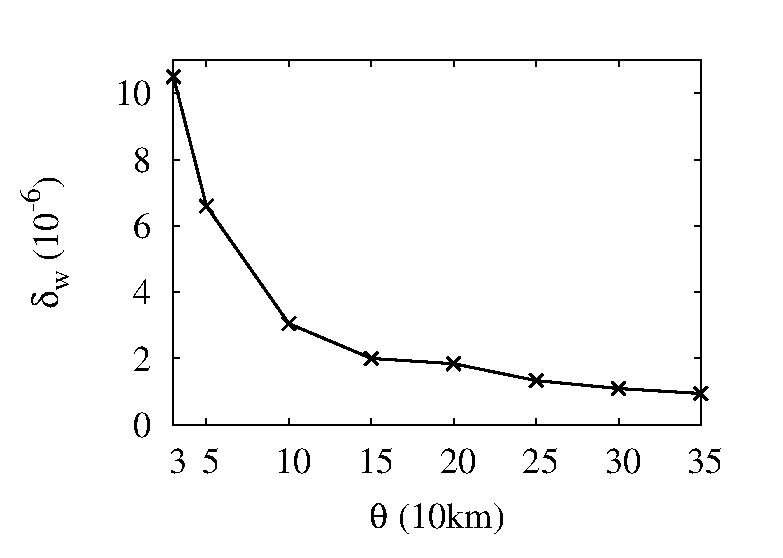
\epsfig{file=images/mdelta.eps,width=0.45\columnwidth}
}
\subfigure[Different Crop Ratio]{
  \label{fig:m}
  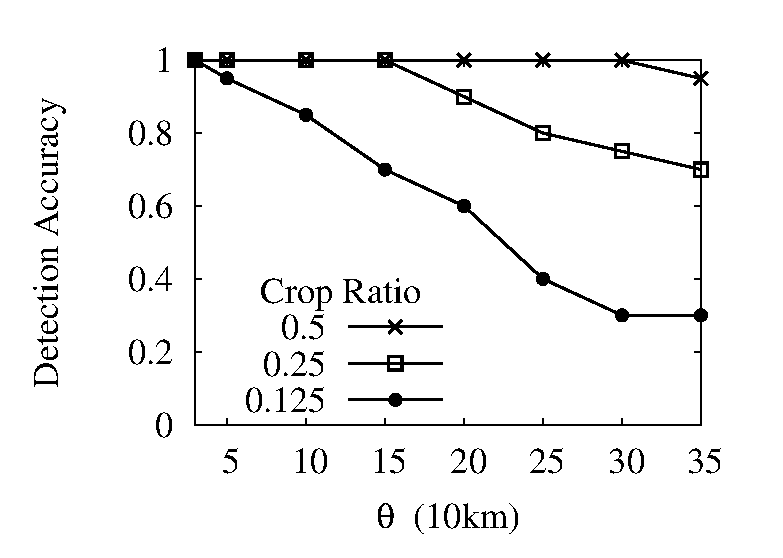
\epsfig{file=images/mparameter.eps,width=0.45\columnwidth}
}
\subfigure[Time of Insertion]{
  \label{fig:ti}
  \epsfig{file=images/time.eps,width=0.45\columnwidth}
}
\subfigure[Time of Detection]{
  \label{fig:td}
  \epsfig{file=images/time1.eps,width=0.45\columnwidth}
}
\caption{Experiment Results under Different Distortion}
\label{fig:pudd}
\end{figure}

%\begin{table}[th]
%\centering
%\caption{Distortion Added by Watermarking}
%\label{tab:dis}
%\begin{tabular}{|c||c|c|c|c|c|c|c|c|} 
%\hline
%$\theta$(km) & 3 & 5 & 10 & 15 & 20 & 25 & 30 & 35 \\\hline \hline
%$\delta (10^{-6})$ & 10.50 & 6.60 & 3.05 & 2.00 & 1.84 & 1.33 & 1.09 & 0.94 \\\hline
%\end{tabular}
%\end{table}

In the following experiment, we watermark a map with certain distortion, here we set 
$\theta =30,000$. After that we crop different ratio from the map to evaluate the performance 
of our algorithm. For each crop ratio, we select different parts of the map to detect 
up to 20 times. We randomly select different parts of the watermarked map to detect (see 
Figure \ref{fig:cropmethod}) and calculate the detection accuracy. Here we also implement 
Voigt's and Pu's methods to make a comparison. Distortion $\delta_w$ added by the watermarking 
is $10.5\times 10^{ -6 }$ (Jiang), $10.8\times 10^{-6}$ (Voigt) and $9.8\times 10^{-6}$ (Pu). 
The distortion of all three methods are almost at the same level.
Figure \ref{fig:cropattack} gives the results.

%\begin{figure}[th]
%\centering
%\subfigure[Time of Insertion]{
%  \label{fig:ti}
%  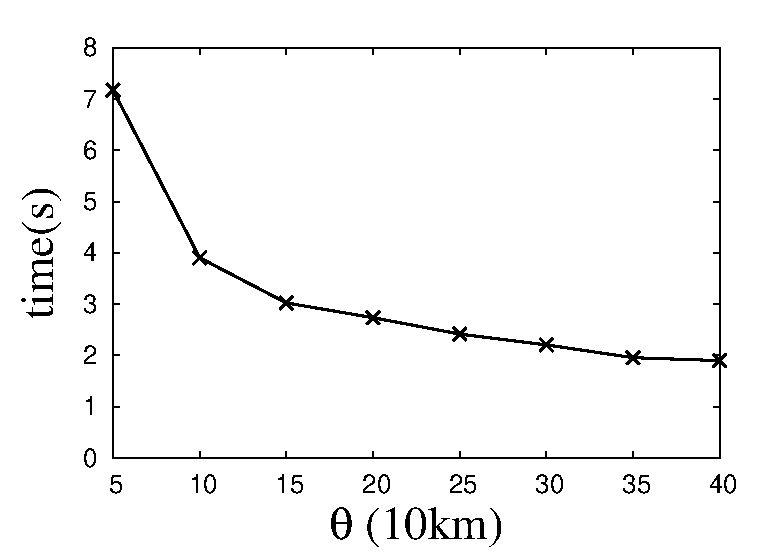
\epsfig{file=time.eps,width=0.45\columnwidth}
%}
%\subfigure[Time of Detection]{
%  \label{fig:td}
%  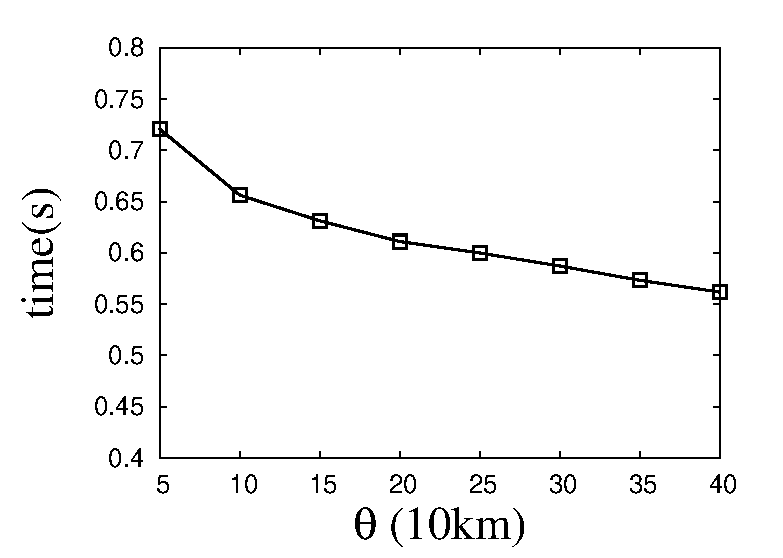
\epsfig{file=time1.eps,width=0.45\columnwidth}
%}
%\caption{Experimental Time Results}
%\label{fig:results}
%\end{figure}

%\begin{figure}[th]
%\centering
%\epsfig{file=cropattack.eps,width=0.7\columnwidth}
%\caption{Performance Under Different Crop Ratio}
%\label{fig:cropattack}
%\end{figure}

\begin{figure}[h]
\centering
\subfigure[\scriptsize Performance under Cropping]{
  \label{fig:cropattack}
  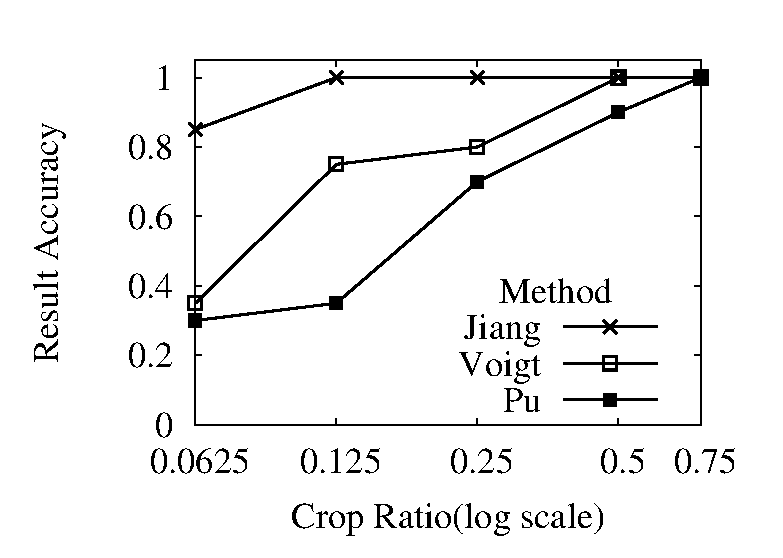
\epsfig{file=images/cropattack.eps,width=0.47\columnwidth}
}
\subfigure[\scriptsize Accuracy in $1/8$ crop ratio]{
  \label{fig:mdelta}
  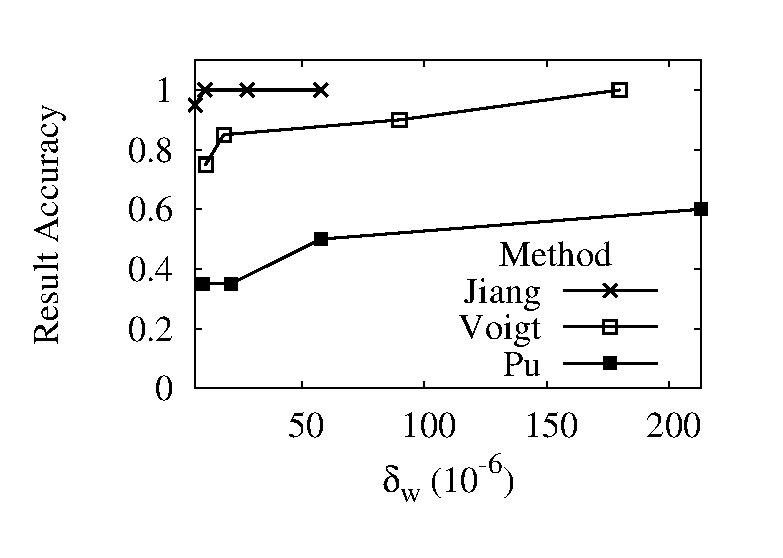
\epsfig{file=images/delta.eps,width=0.47\columnwidth}
}
\caption{Performance under Crop Attack}
\end{figure}

According to the experiment result, we can find that our algorithm keeps a perfect
result when the crop ratio is up to $1/8$, while the comparison methods show a significant
accuracy degradation. And when crop ratio is $1/16$, we still contain a high accuracy.
We also test the detection accuracy under different distortion in $1/8$ crop ratio
(see Figure \ref{fig:mdelta}). In this experiment, our algorithm can attain
a $100\%$ detection accuracy with just little distortion. Since the detection accuracy of 
our algorithm quickly attain to $1$, it is not necessary to plot too many points in Figure 
\ref{fig:mdelta}.

%\begin{figure}[h]
%\centering
%\epsfig{file=delta.eps,width=0.7\columnwidth}
%\caption{Detection Accuracy in $1/8$ crop ratio}
%\label{fig:mdelta}
%\end{figure}

\subsection{Performance under Merge Attack}
%\JK{For merge part, I plan to design two experiments:\\
%1).I plan to watermark a map with the same distortion distance as crop 3) and 
%make a merge map like figure \ref{fig:merge}. What I want to show the readers is
%a direct result of the merge detection result: suspicious regions and detection
%confidence. A visual figure can also be drawn.\\
%2).Just like merge 3), I plan to crop the watermarked map into different ratio
%and merge with the other data source to make different maps, for each ratio, 20
%different merge maps will be detected. The result will be a ``Detection accuracy-
%watermarked ratio''figure for all three algorithms.} 

%\KZ{So (1) is a special case of (2) which is actually fig 15 right? For
%(1) you will just have a detection number for 3 algorithms? I think you can
%show visually what was the original merge situation and what was the 
%portion that you detected by comparing and contrasting the difference in
%a figure. That will be visually impactful.}

In this experiment, we select the $2012$ TIGER map of Minneapolis-St. Paul 
Metropolitan area as another data source, which can be downloaded from the 
United States Census Website\cite{tigerurl}. The coordinate system of TIGER 
map is different from MN dot base Map. We transform the coordinate system of 
TIGER map to make it same as the former data source. Figure \ref{fig:17} is 
the overlap of these two maps of Anoka county after the synchronization. 
%As we can see that very slight difference could be found between these two maps, 
%so we have a good reason to believe that if we implement our partition algorithm 
%on a merge map of them, the result will almost be the same.


\begin{figure}[th]
\centering
\epsfig{file=images/overlap.eps,width=0.7\columnwidth}
\caption{Overlap of Two Maps}
\label{fig:17}
\end{figure}
We crop a watermarked map ($\delta_w = 6.60 \times 10^{-6}$) and merge part of it with TIGER 
map to make a ``new'' map (see Figure \ref{fig:mattack}). The result of the 
merge detection: suspicious regions and detection confidence is shown in Table 
\ref{tab:merge}. Here we select those regions which have at least 10 points tested. 
From the corresponding visual figure (see Figure \ref{fig:mresult}), we can see 
that our algorithm almost ``exactly'' decides the suspicious regions. 

\begin{figure}[h]
\centering
\subfigure[\scriptsize Merge Attack]{
  \label{fig:mattack}
  \epsfig{file=images/mattack.eps,width=0.42\columnwidth}
}
\subfigure[\scriptsize Detection Result]{
  \label{fig:mresult}
  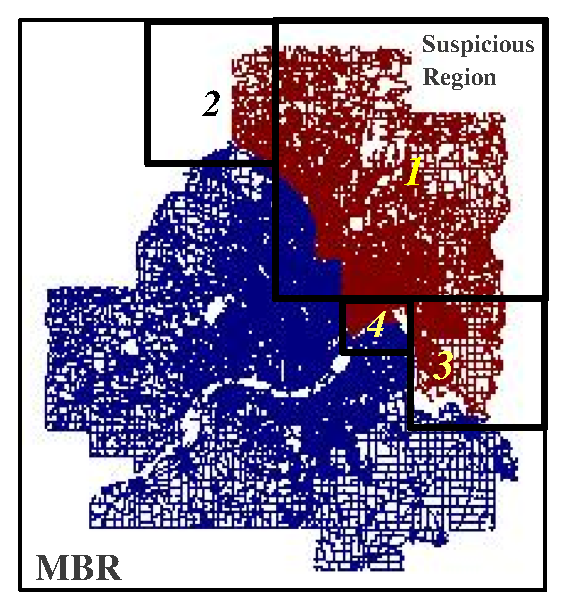
\epsfig{file=images/mresult.eps,width=0.42\columnwidth}
}
\caption{Merged Map}
\end{figure}

%\begin{figure}[th]
%\centering
%\epsfig{file=merge.eps,width=0.8\columnwidth}
%\caption{Merged Map}
%\label{fig:mergeexp1}
%\end{figure}


\begin{table}[th]
\centering
\caption{Merge Attack Detection}
\label{tab:merge}
\begin{tabular}{|c||c|c|c|c|} 
\hline
Region & Total & Match & Confidence & Result \\\hline \hline
1 & 147 & 122 & 1.000 & positive\\\hline
2 & 12 & 11 & 0.997 & positive\\\hline
3 & 23 & 18 & 0.994 & positive\\\hline
4 & 15 & 12 & 0.983 & positive\\\hline
\end{tabular}
\end{table}

We also watermark the Minneapolis-St. Paul Metropolitan area and then split this 
watermarked map into the same small portions as cropping experiment above. After 
that we merge these maps with the complementary parts of map from TIGER to create 
some new digital road maps. In this experiment, we also implement the two other 
method to make a comparison. Distortion $\delta_w$ added by the watermarking still
is $10.5\times 10^{ -6 }$ (Jiang), $10.8\times 10^{-6}$ (Voigt) and $9.8\times 10^{-6}$ (Pu). 
Figure \ref{fig:mergeattack} shows the result of our 
experiments.

%\begin{figure}[th]
%\centering
%\epsfig{file=mergeattack.eps,width=0.7\columnwidth}
%\caption{Performance Under Merge Attack}
%\label{fig:mergeattack}
%\end{figure}

\begin{figure}[h]
\centering
\subfigure[\scriptsize Performance under merging]{
  \label{fig:mergeattack}
  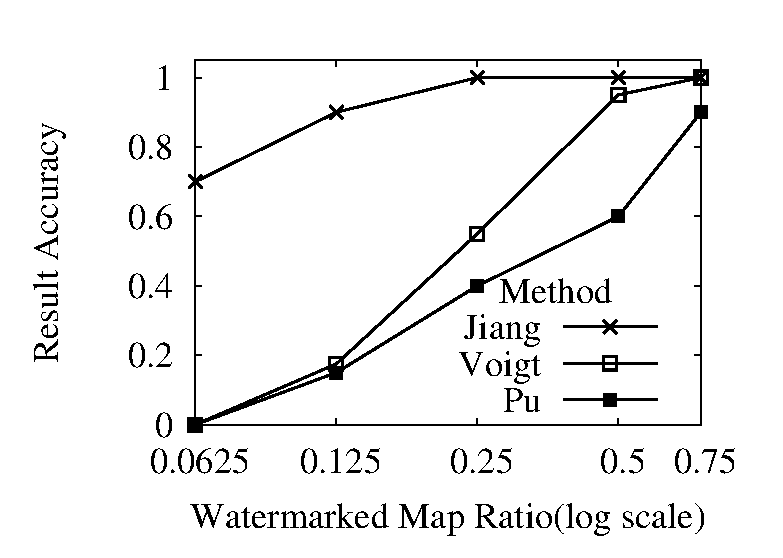
\epsfig{file=images/mergeattack.eps,width=0.47\columnwidth}
}
\subfigure[\scriptsize Accuracy in $1/8$ merge ratio]{
  \label{fig:deltamerge}
  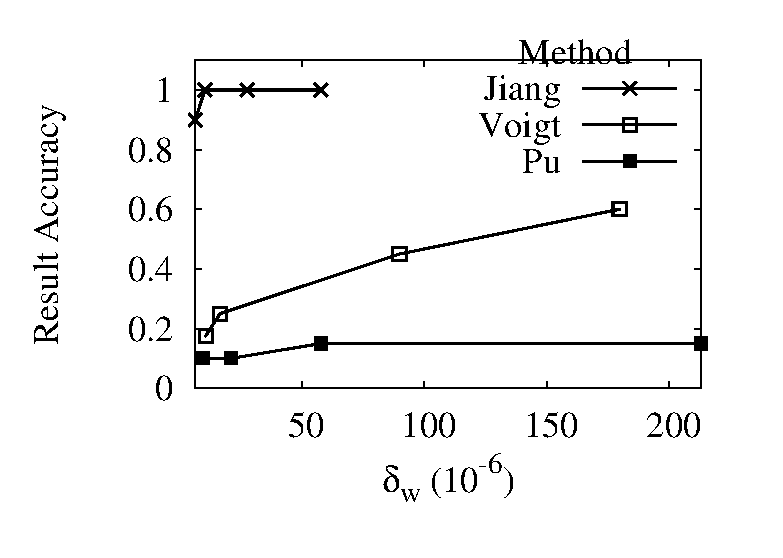
\epsfig{file=images/deltamerge.eps,width=0.47\columnwidth}
}
\caption{Performance under Merge Attack}
\end{figure}

Comparing with the cropping experiment, we can obviously find the performance of 
our proposed algorithm is almost not affected by the complementary part of the map. 
However, the detection accuracy of the other two methods decrease significantly. 
The reason is the complementary map provides sufficient disturb to watermarked data.
Similarly, we also implement another experiment to evaluate the relationship between
detection accuracy and watermark distortion $\delta_w$. From this figure, we can see that
our algorithm still can quickly attain a quite high detection accuracy. However, when 
$\delta_w$ increases for Pu's and Voigt's method, the detection accuracy doesn't changed significantly.
The reason for Pu should be that it's global liner correlation is destroyed by ``merge'' attack.
For Voigt's method, though more watermark information is used for detection, more ``merge'' 
noise will will also be added to the detection process. Thus increase of detection accuracy
for them is not significant.



%\begin{figure}[h]
%\centering
%\epsfig{file=deltamerge.eps,width=0.7\columnwidth}
%\caption{Detection Accuracy in $1/8$ Merge ratio}
%\label{fig:deltamerge}
%\end{figure}



%%% Local Variables:
%%% mode: latex
%%% TeX-master: "paper"
%%% End:
